\newpage

\section{Github + Travis CI mittels arara + luatex}
\subsection{aktuelle Probleme}
\subsubsection{Linux}
\begin{itemize}
  \item Travis CI verwende eine sehr alte Ubuntu-Version.\\ (Dadurch nur eine veraltete TexLive installation\\ $\Rightarrow$ hinderlich bei Lua\TeX)
  \item Aktuell verfügbare Docker-Container bekommen \\das Texlive Update nicht hin.
  \item Arara bekommt generell keine Rechte um die Dateien zu schreiben. \\
  (Evtl. lösbar, aber die Zeit ist grade knapp)
\end{itemize}

\newpage
$\Rightarrow$ aktuelle Probleme
\subsubsection{MacOS 10}
\begin{itemize}
  \item Unter OSX dauert die Latex Installation zu lange. \\ $\Rightarrow$ Travis CI bricht ab ...
  \item Docker-Nutzung schwierig, da man dafür Virtualbox + ein Linux benötigt.
  \item Brew (Ein Paketmanager für MacOS) enthält kein Tex-Live.
  \item Macports (nicht in den TravisCI - macOS10-Installationen enthalten)
\end{itemize}


\newpage % ============================================= Newpage ===================

\monocodebox{latex}{Was benötigt es für arara:}{./nopTex.tex}{true}{1}{3}

\monocodebox{sh}{Hinzufuegen der nötigen Änderungen}{./code/travis.sh}{true}{80}{80}







%
% \begin{figure}[ht]
%   \section{arara + lua \TeX}
% \adjustbox{valign=t}{\begin{minipage}[t]{0.50\textwidth}
% \begin{framed}
%   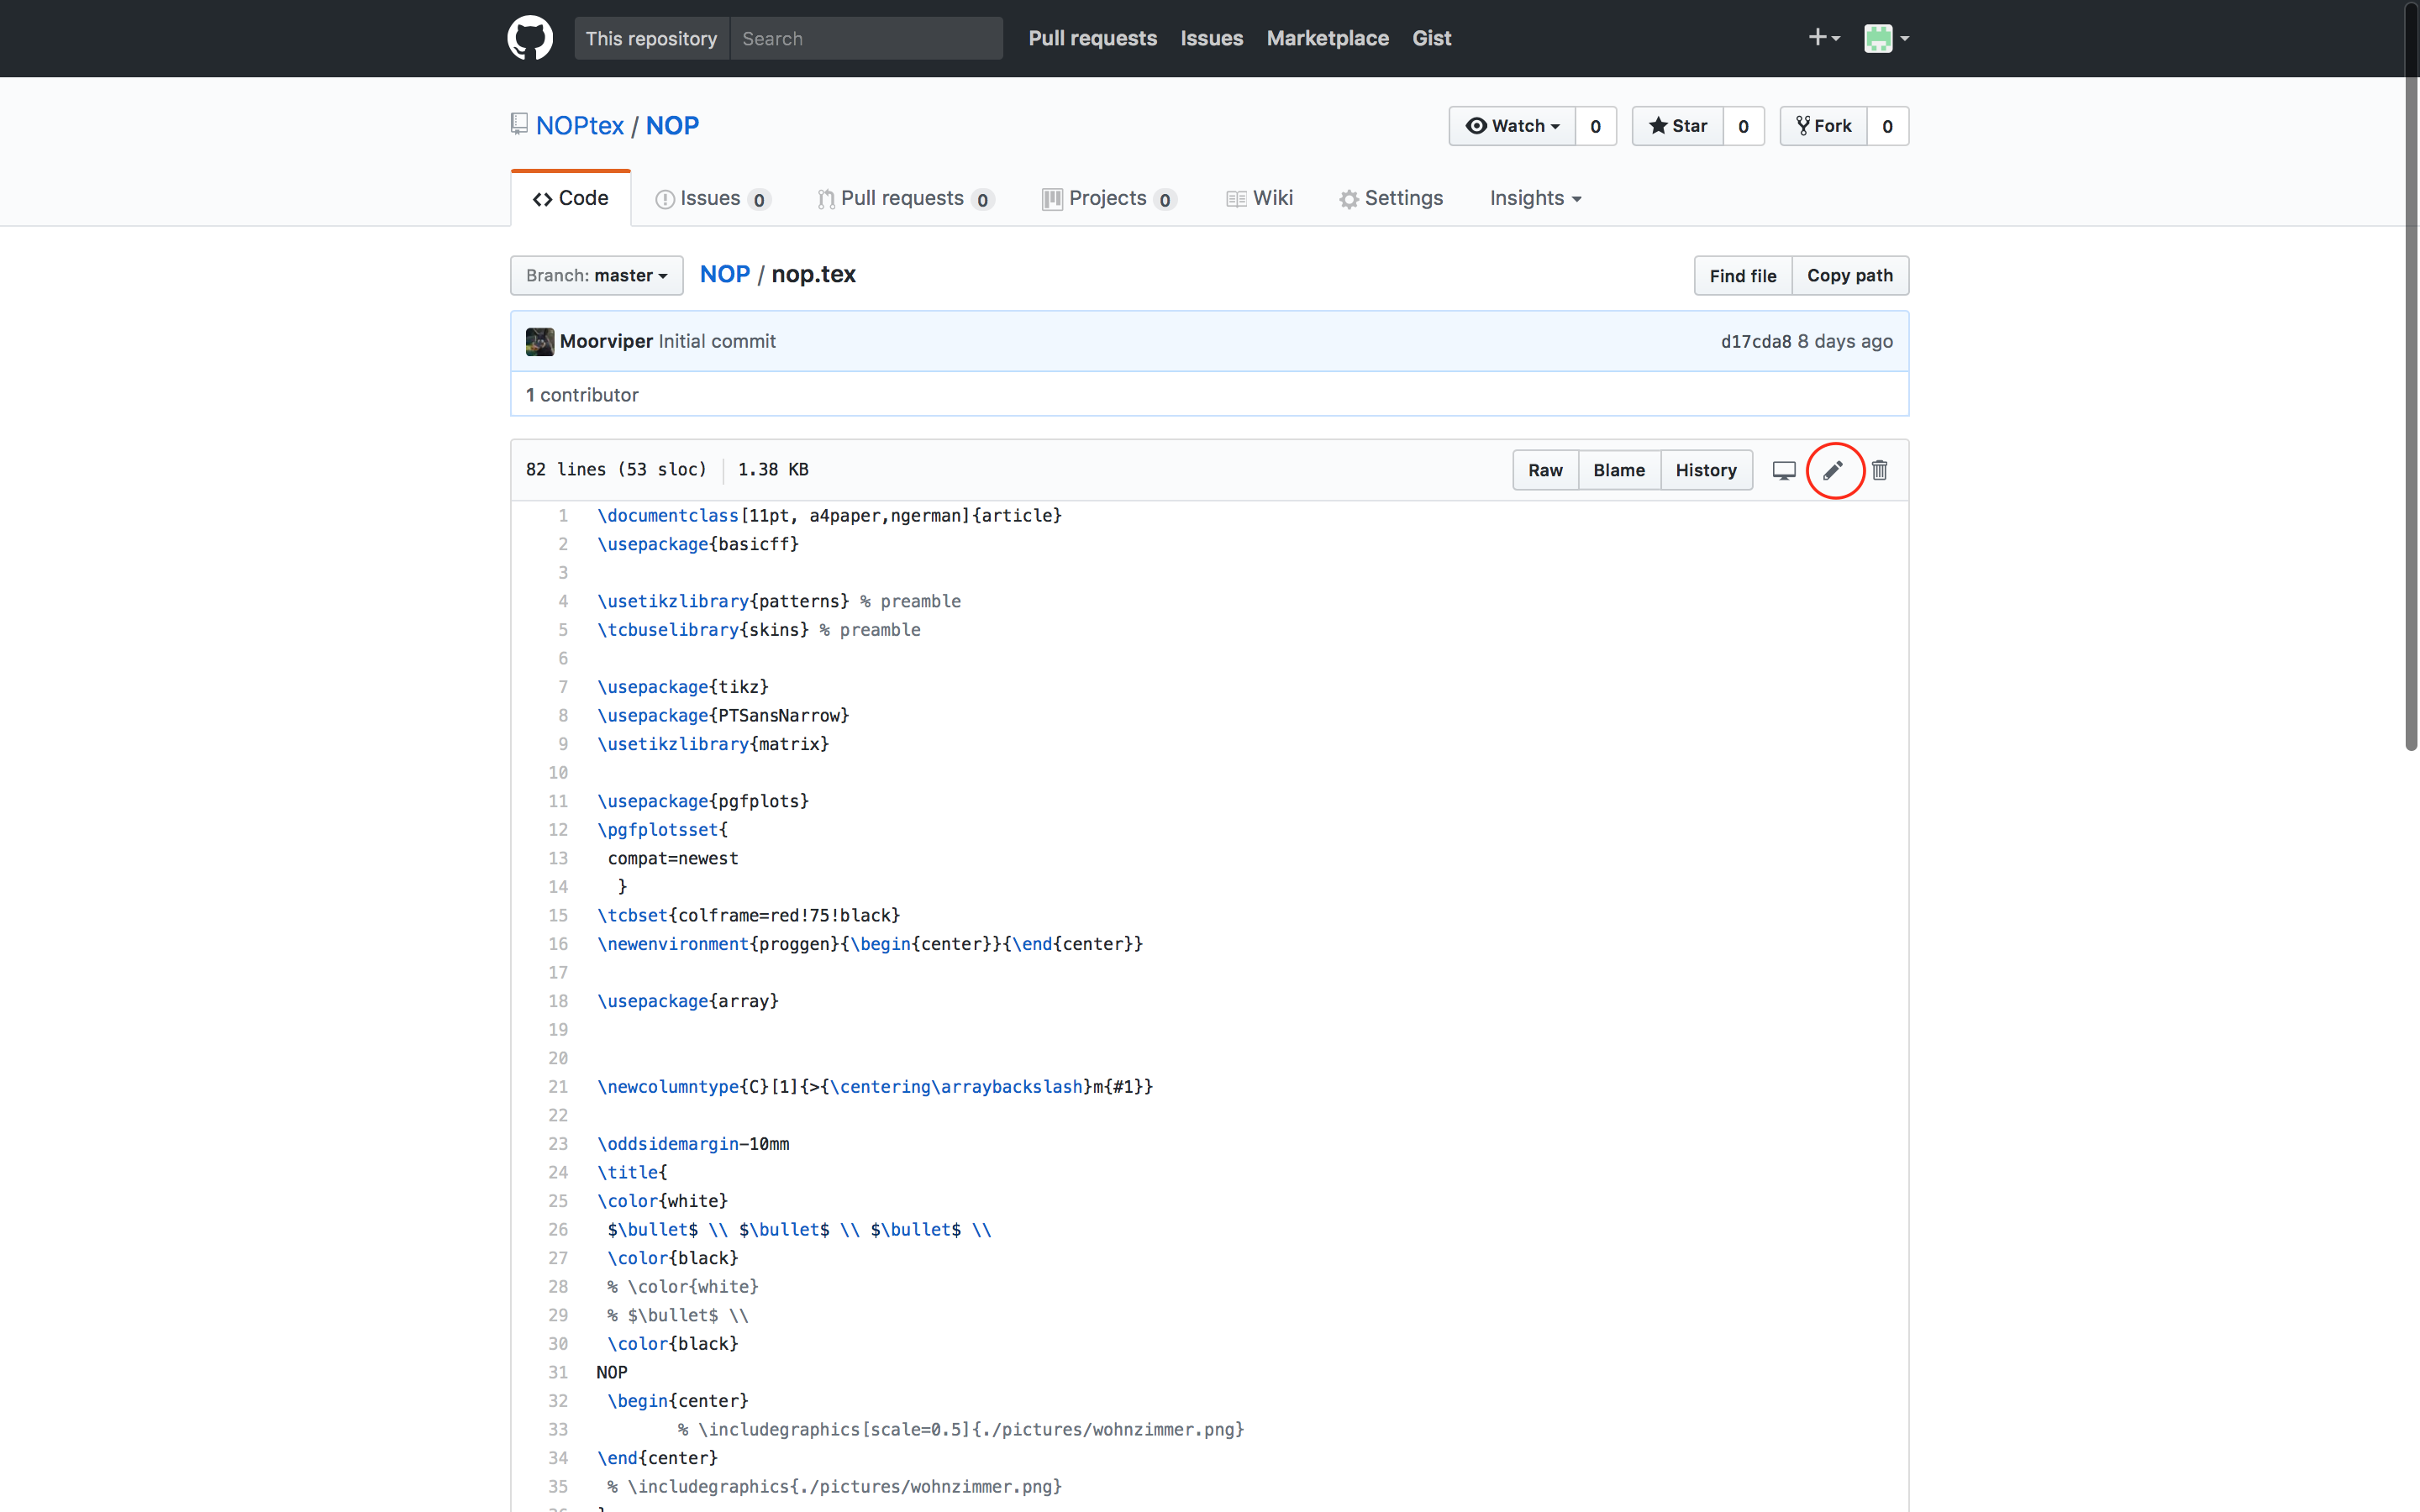
\includegraphics[width=1.0\textwidth]{./bilder/21edit.png}
% \end{framed}
%
% \end{minipage}}
% % \hfill
% \adjustbox{valign=t}{\begin{minipage}[t]{0.45\textwidth}
% \vspace{0pt}
% \huge
% Man klickt auf den Stift zum editieren der Datei.
% % \caption{Kapazität}
% \end{minipage}}
% % \end{figure}
% % \vspace{0.5cm} % ----------------------------------- vspace
% % \begin{figure}[ht]
% \adjustbox{valign=t}{\begin{minipage}[t]{0.50\textwidth}
% % \vspace{0.5cm}
% \begin{framed}
%   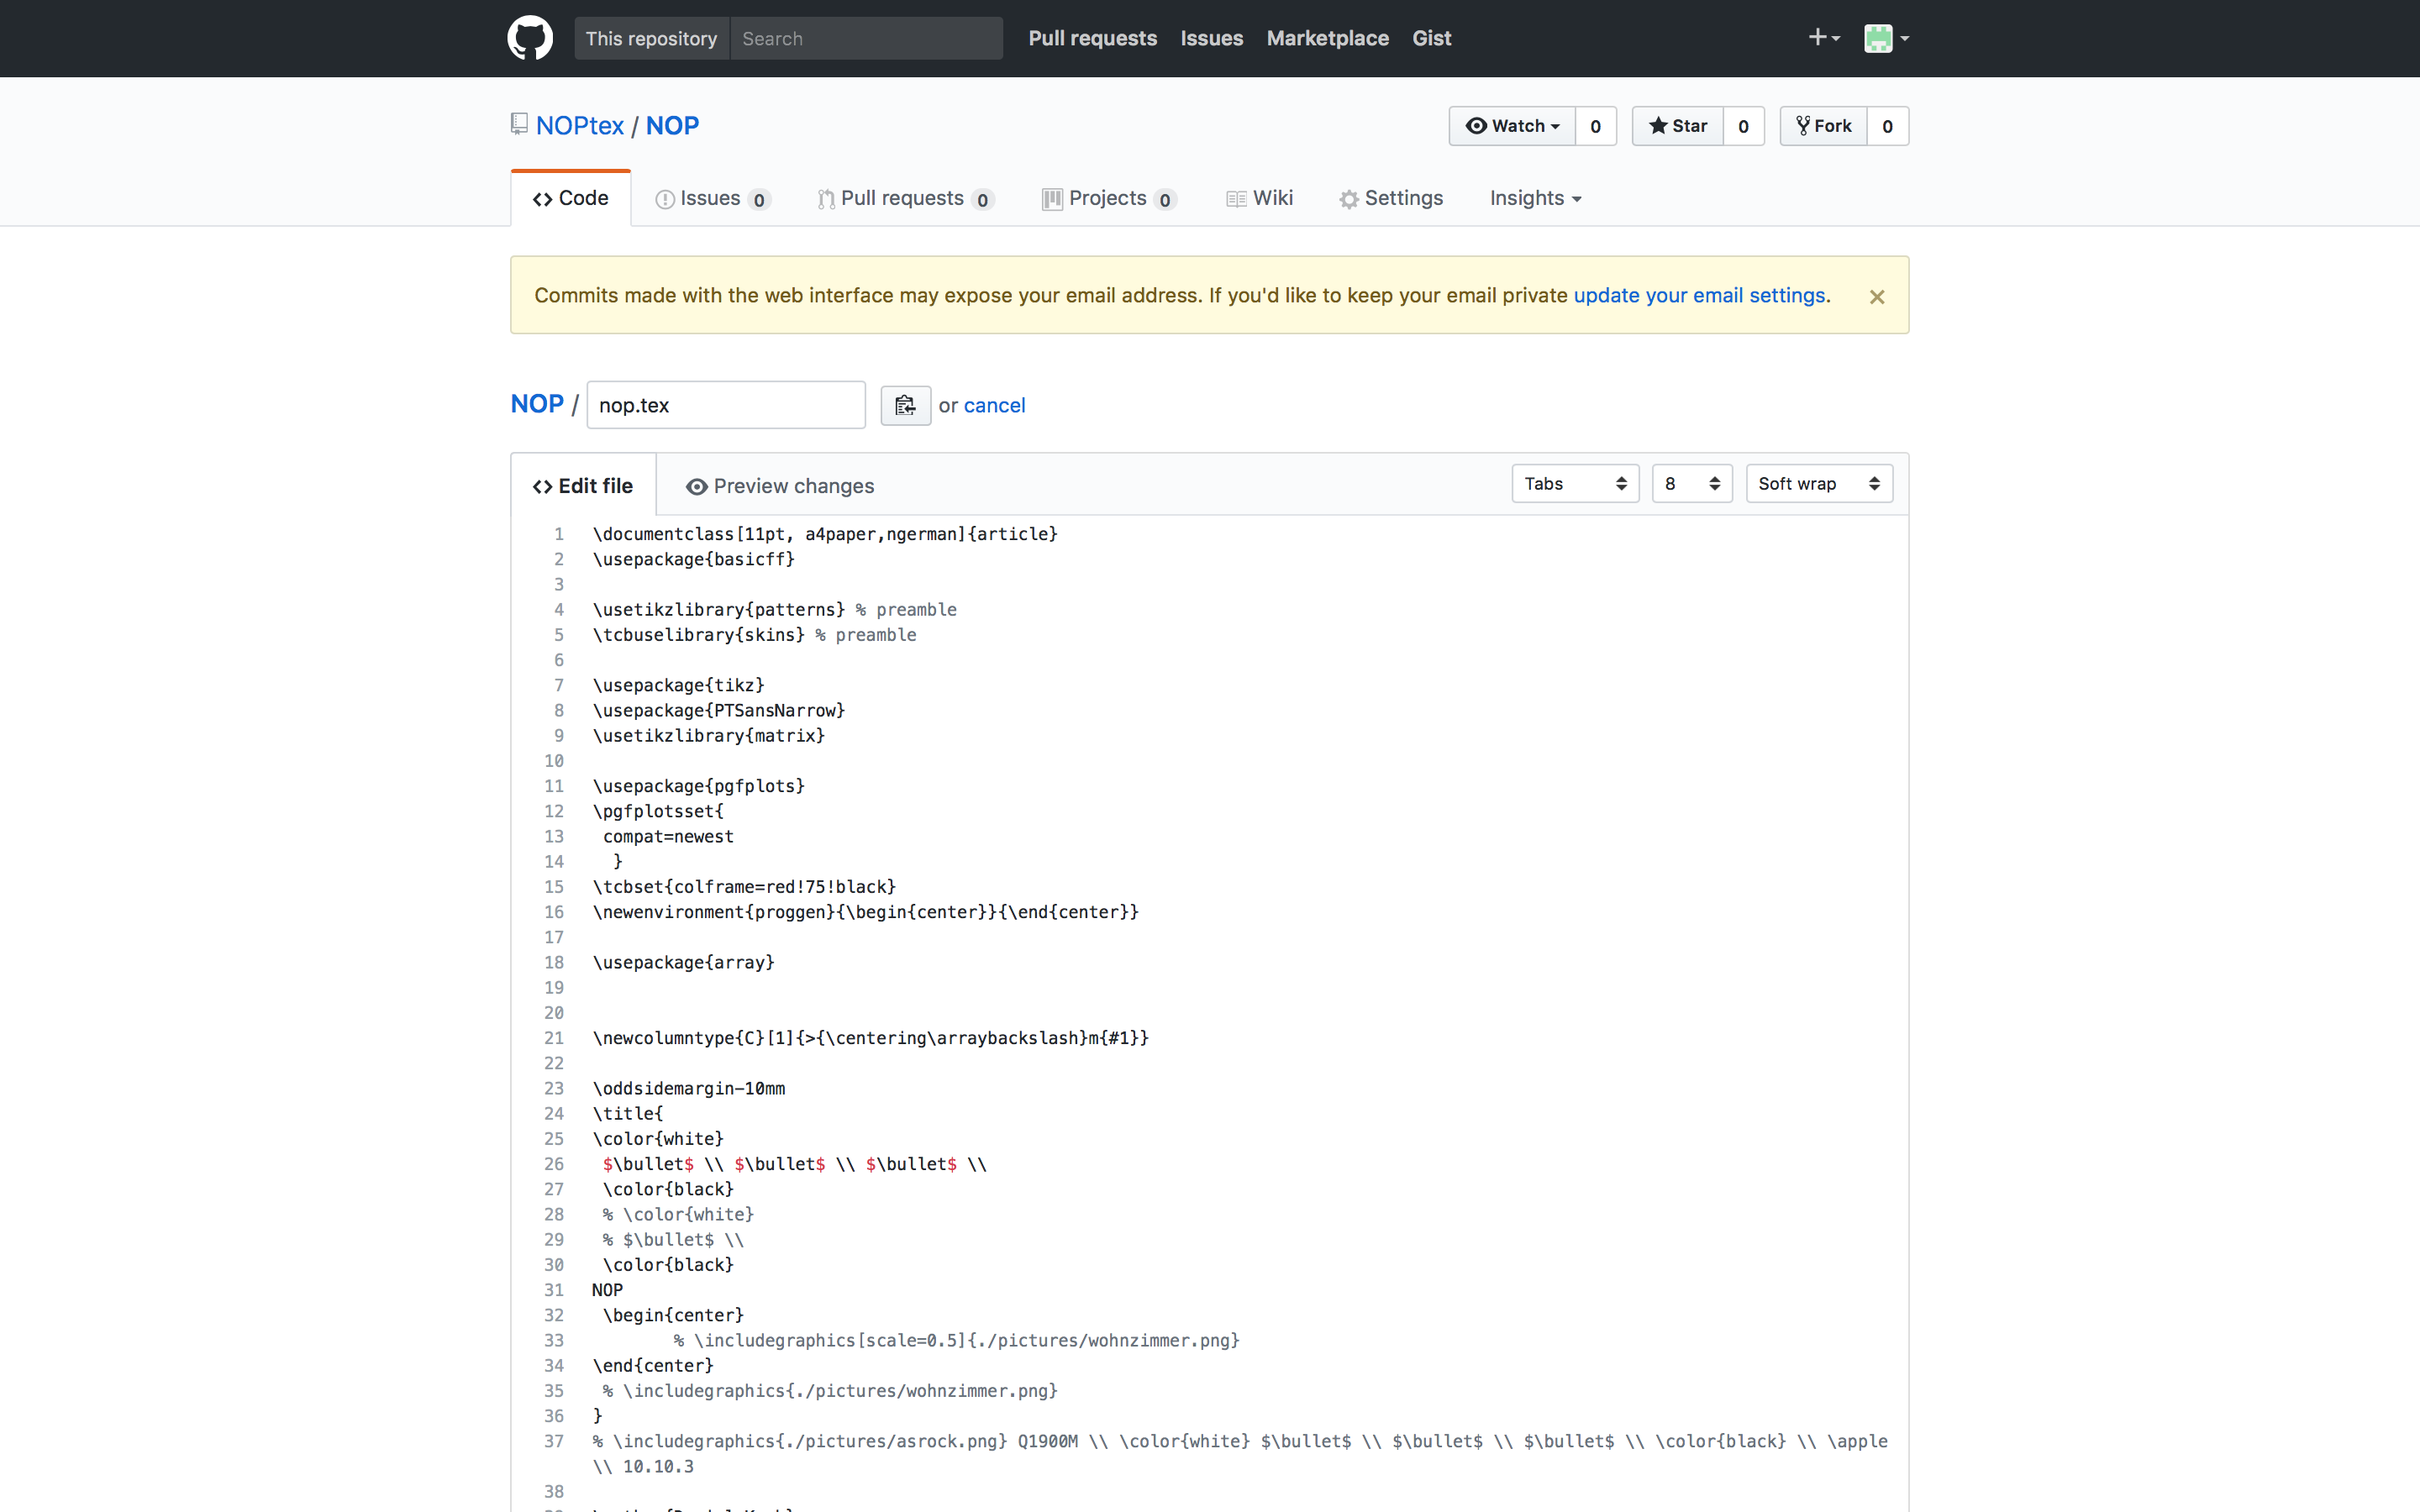
\includegraphics[width=1.0\textwidth]{./bilder/22edit.png}
% \end{framed}
%
% \end{minipage}}
% \hfill
% \adjustbox{valign=t}{\begin{minipage}[t]{0.45\textwidth}
% \vspace{0pt}
% \huge
% Die Anzeige ändert sich geringfüging.
% % \caption{Kapazität}
% \end{minipage}}
% \end{figure}
%
% \clearpage % GleitObjekte anzeigen



\newpage

\textbf{Wie gehts weiter / Nächste Schritte :}
\begin{itemize}
  \item Macports sauber auf macOS El Capitan installieren
  \item Texlive sauber installieren
  \item Rechte ordentlich setzen
\end{itemize}

\textbf{Dann baut es hoffentlich}
%
%
% \begin{figure}[]
%   \subsubsection{Github Repo mit Travis CI verbinden}
% \adjustbox{valign=t}{\begin{minipage}[t]{0.50\textwidth}
% \begin{framed}
%   \includegraphics[width=1.0\textwidth]{./bilder/1gitRepoSettings.png}
% \end{framed}
%
% \end{minipage}}
% % \hfill
% \adjustbox{valign=t}{\begin{minipage}[t]{0.5\textwidth}
% \vspace{0pt}
% \huge
% Im Repo klickt man auf Settings
% % \caption{Kapazität}
% \end{minipage}}
% % \end{figure}
% % \vspace{0.5cm} % ----------------------------------- vspace
% % \begin{figure}[ht]
% \adjustbox{valign=t}{\begin{minipage}[t]{0.40\textwidth}
% % \vspace{0.5cm}
% \begin{framed}
%   \includegraphics[width=1.0\textwidth]{./bilder/2integrationServices.png}
% \end{framed}
%
% \end{minipage}}
% \hfill
% \adjustbox{valign=t}{\begin{minipage}[t]{0.43\textwidth}
% \vspace{0pt}
% \huge
% Danach
% % \caption{Kapazität}
% \end{minipage}}
% \end{figure}
%
% \clearpage % GleitObjekte anzeigen
% \newpage
% \begin{table}
%   \caption{title}
% \end{table}
% Test


% \begin{center}
%  % \includegraphics[scale=0.5]{./pictures/wohnzimmer.png}
% \end{center}
% \begin{figure}
%     \subfigure[Bezeichnung der linken Grafik]{\includegraphics[width=0.49\textwidth]{./bilder/1gitRepoSettings.png}}
%     \subfigure[Bezeichnung der rechten Grafik]{\includegraphics[width=0.49\textwidth]{./bilder/2integrationServices.png}}
% \caption{Titel unterm gesamten Bild}
% \end{figure}


% \begin{figure}
%     \subfigure[Bezeichnung der linken Grafik]{\includegraphics[width=0.49\textwidth]{./bilder/1gitRepoSettings.png}}
%     \subfigure[Bezeichnung der rechten Grafik]{Test tesxt}
% \caption{Titel unterm gesamten Bild}
% \end{figure}










% \newpage
%
% \newpage
% bla
% \newpage
% bla
% \newpage
%
% \begin{figure}[ht]
% \adjustbox{valign=t}{\begin{minipage}[t]{0.66\textwidth}
% \includegraphics[width=1.0\textwidth]{./bilder/1gitRepoSettings.png}
% \end{minipage}}
% \hfill
% \adjustbox{valign=t}{\begin{minipage}[t]{150pt}
% \vspace{0pt}
% \huge
%
% % \caption{Kapazität}
% \end{minipage}}
% \end{figure}
%
% 3.1. Setup Github repo
% \newpage
% If you have forked this repo, then directly go to Settings option, otherwise, first create a new repository on Github and then, then go to Settings option of your repository.
% Click on Webhooks und Services and then Add service
% Select Travis CI
% Add your Travis CI username and Token
% Add service
% 3.2. Setup Travis CI
%
% Go to Travis CI
% Toggle on your repository
% 3.3. Install Travis Command-line Tool
%
% To configure Travis build to deploy generated PDF to Github releases, we have to get Github OAuth Token. To get it and securely embed it into .travis.yml file, we have to install Travis Command-line Tool
%
% gem install travis -v 1.7.5 --no-rdoc --no-ri
% travis setup releases
% Provide your Github username and password, to generate token and encrypt it on the go. This will also add it to your .travis.yml file.
